%%%%%%%%%%%%%%%%%%%%%%%%%%%%%%%%%%%%%%%%%%%%%%%%%%%%%%%%%%%%%%%%%%%%%%%%%%%%
\documentclass{beamer}           % pdfTeX の場合
% 付録をページ数にカウントしない NPC
\usepackage[orientation=portrait,size=a0,scale=1.5]{beamerposter}% whole 指定
\setbeamertemplate{navigation symbols}{} % ナビゲーションを消す
\usefonttheme{professionalfonts} % 数式のフォントをかっこよくする

\usepackage[at]{easylist}
\usepackage[whole]{bxcjkjatype}% whole 指定
\usepackage{algorithm}
\usepackage{tcolorbox}
\usepackage{algorithmic}
%\usepackage{theorem}
\usepackage{bm}
\usepackage{amsthm}
\usepackage{amsmath}
\usepackage{bbm}
%\usepackage[dvipdfmx]{graphicx}
\usepackage{graphicx}
\usepackage{overpic}
\usepackage{wrapfig}
\usepackage[overlay]{textpos}
%\setbeamertemplate{background}[grid][step=30pt]
\usepackage{stackengine} % for addstackgap

\newcommand{\bhrule}{{\color{blue} \hrule}}

\definecolor{nico}{rgb}{1, 0.90, 0.96}
\definecolor{red}{rgb}{1.0, 0.0, 0.0}
\definecolor{orange}{rgb}{0.95, 0.3, 0.0}
\definecolor{green}{rgb}{0.0, 0.5, 0.0}
\definecolor{ash}{rgb}{0.4,0.4,0.4}
\definecolor{myblue}{rgb}{0.2,0.2,0.7}
\setbeamercolor{mine}{fg=white,bg=blue!70!cyan}
\renewcommand{\alert}[1]{{\color{red} {#1}}}
\renewcommand{\structure}[1]{{\color{blue!50!cyan} {#1} }}
\tcbset{colframe=myblue,colback=white,boxsep=16px} % textcolorbox settings

\newcommand{\express}[1]{{\color{green} {#1}}}
\newcommand{\p}{\textcolor{blue}{+1}}
\newcommand{\m}{\textcolor{red}{-1}}
\newcommand{\prop}[1]{\rule[0mm]{0mm}{#1}}
\newcommand{\TSS}{\mathrm{TSS}}
\newcommand{\mymin}[1]{\min_{\scalebox{1.0}{$#1$}}}
\newcommand{\X}[1]{X_{\scalebox{0.9}{$#1$}}}
\newcommand{\A}[1]{A_{\scalebox{0.9}{$#1$}}}
\renewcommand{\a}{\bar{a}}
\renewcommand{\b}{\bar{b}}
\newcommand{\mysum}[1]{\sum_{i=0}^{#1}}

\newlength{\graphwidth}
\setlength{\graphwidth}{130pt}

%% thick hline
\makeatletter
\def\thickhline{%
  \noalign{\ifnum0=`}\fi\hrule \@height \thickarrayrulewidth \futurelet
   \reserved@a\@xthickhline}
\def\@xthickhline{\ifx\reserved@a\thickhline
               \vskip\doublerulesep
               \vskip-\thickarrayrulewidth
             \fi
      \ifnum0=`{\fi}}
\makeatother

\newlength{\thickarrayrulewidth}
\setlength{\thickarrayrulewidth}{2\arrayrulewidth}

%% command set for circled graph notations
%\renewcommand{\v}[1]{\textcircled{\raisebox{-0.7pt}{\footnotesize{#1}}}}
\renewcommand{\v}[1]{\textcircled{\raisebox{-0.7pt}{\footnotesize{#1}}}}
\newcommand{\e}{\text{--}}

%% for linear nonlinear
\newcommand{\gxxx}[3]{\v{#1}\e\v{#2}\e\v{#3}}

%% for stackengine
\renewcommand{\ss}[2]{\addstackgap{\shortstack{#1\\#2}}}

%% for acc table
%\renewcommand{\*}[1]{\hspace{5pt}#1\raisebox{2pt}{\scriptsize *}}
\newcommand{\fst}[1]{{\bf #1}}
\newcommand{\fss}[2]{\addstackgap{\shortstack{\bf #1\\#2}}}

%TODO 黄色をポスター印刷機用にもっと明るくする
\title{\fontsize{65pt}{0pt} \selectfont 適応的な部分グラフ指示子の探索・選択に基づく非線形グラフ分類回帰}
\author{\large 白川 稜, 横山 侑政, 岡崎 文哉, 瀧川 一学 ~~~北海道大学 \fontsize{40pt}{0pt} \selectfont~email:sira@ist.hokudai.ac.jp}

%%%%%%%%%%%%%%%%%%%%%%%%%%%%%%%%%%%%%%%%%%%%%%%%%%%%%%%%%%%%%%%%%%%%%%%%%%%

\setbeamercolor{myframetitle}{fg=white,bg=myblue}

\begin{document}
~ \\
\begin{beamercolorbox}[
    wd=\textwidth,
    sep=0pt,     % パディング 2pt
]{myframetitle}
\begin{center}
	\vspace{20pt}
	{\inserttitle} \\
	%{\fontsize{65pt}{0pt} \selectfont \inserttitle} \\
	\vspace{10pt}
	\medskip
	\medskip
	{\insertauthor} \\
	\vspace{20pt}
\end{center}
\end{beamercolorbox}

\vspace{-20pt}
\begin{columns}[T]
	\begin{column}{0.50\textwidth}
		\begin{tcolorbox}[title={\large 概要}]
	\begin{easylist}[itemize]
			@ グラフに対する教師付き学習(分類・回帰)
			\vspace{10pt}
			@ 特徴量に部分グラフ指示子を利用
			\vspace{10pt}
			@ 部分グラフの総数は膨大、全列挙困難
			\vspace{10pt}
			@ 特徴探索及びモデル構築の同時学習
			\vspace{10pt}
			@ モンテカルロ木探索を利用した効率的な部分グラフ指示子の探索・選択
			\vspace{10pt}
			@ 回帰木勾配ブースティングによる非線形モデルの構築
		\end{easylist}
	\end{tcolorbox}

		\begin{tcolorbox}[title={\Large 背景}]
	\structure{グラフ}は広く用いられる重要なデータ構造
	\begin{easylist}[itemize]
	@ 化学構造式
	@ RNA二次構造
	@ 構文木 \\
	\end{easylist}
	\vspace{-20pt}

	\structure{グラフに対する教師付き学習}
	\begin{easylist}[itemize]
	@ 様々な分野での応用
	@@ 創薬
	@@ 材料科学
	\end{easylist}
	\begin{textblock*}{\textwidth}(520pt,-200pt)
		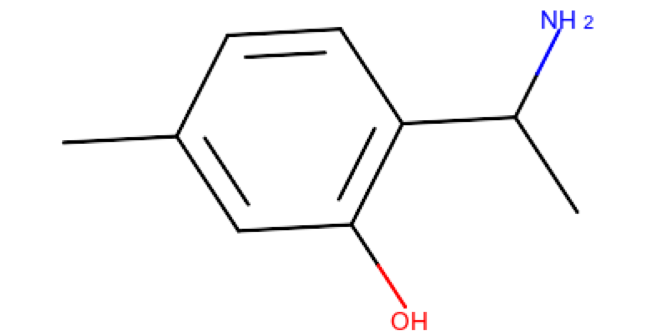
\includegraphics[width=320pt]{img/chemical.png}
	\end{textblock*}
	\begin{textblock*}{\textwidth}(850pt,-200pt)
		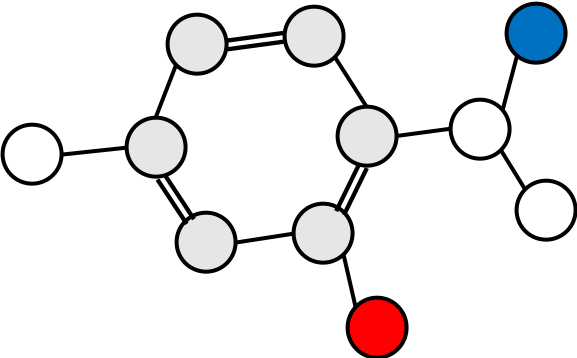
\includegraphics[width=250pt]{img/chemical_graph.png}
	\end{textblock*}
\end{tcolorbox}

		\begin{tcolorbox}[title={\large グラフに対する教師付き学習}]
	\structure{入力}ラベル ($y$ : 離散, 実数値) 付きグラフ集合 \\
	\vspace{5pt}
	\begin{center}
		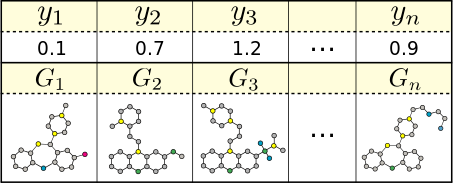
\includegraphics[width=470pt]{img/graph_classify.png}
	\end{center}
	\structure{出力}未知のグラフに対するラベルを予測する予測モデル \\
	\vspace{5pt}\\
	\structure{特徴量}部分グラフ指示子 \\
	\vspace{5pt}
	\begin{center}
		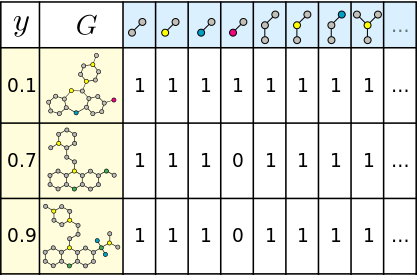
\includegraphics[width=470pt]{img/graph_indicator.png}
	\end{center}
	\vspace{-15pt}
	\structure{既存研究} 
	\begin{easylist}[itemize]
	@ 2-step 手法(Wale+ 2007) \\
	$~~~$ \alert{事前選択された特徴}の列挙 + 任意モデルでの学習 \\
	$~~~~~~~~ \rightarrow$ 事前に選択される特徴に大きく影響
	\vspace{10pt}
	@ gBoost(Saigo+ 2009) \\
	$~~~$ 適応的部分グラフ指示子の探索・選択に基づく\alert{線形}モデル \\
	$~~~~~~~~ \rightarrow$ \express{全部分グラフ指示子}の考慮が可能 \\
	$~~~$ 厳密探索により、\alert{探索コスト大} 
	\end{easylist}
\end{tcolorbox}


	\end{column}
	\begin{column}{0.50\textwidth}
		\begin{tcolorbox}[title={\Large アプローチ}]
	\begin{easylist}[itemize]
	@ branch \& bound手法を用いた特徴探索により\express{全部分グラフ指示子}を考慮した{\bf回帰木の学習}
	@ 精度及び不安定性向上のためアンサンブル学習({\bf 勾配ブースティング})を基にした\express{非線形モデル}の構築
	@ 実験による線形、非線形モデル間の比較
	\end{easylist}
\end{tcolorbox}

		\begin{tcolorbox}[title={\Large 実験&結果}]
	\structure{精度予測(\%) Graph-XOR} \\
		"Graph-XOR": 非線形な学習を要するグラフ版XOR

		\vspace{20pt}
		\begin{figure}[t]
			\scalebox{0.9}{
				\begin{tabular}{c}
					\begin{minipage}{0.3\hsize}
						\centering
						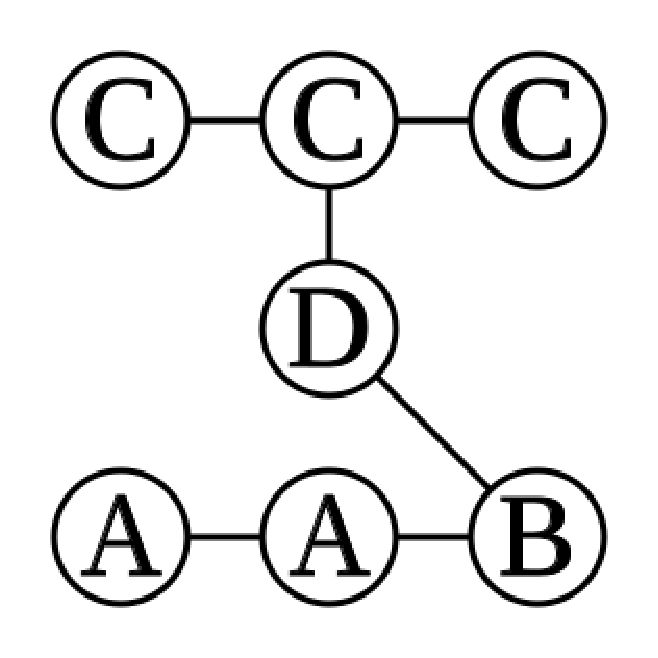
\includegraphics[width=0.4\textwidth]{img/artificial_graph/ccc2aab3.eps} \\
						$y = +1$
					\end{minipage} 
					\begin{minipage}{0.3\hsize}
						\centering
						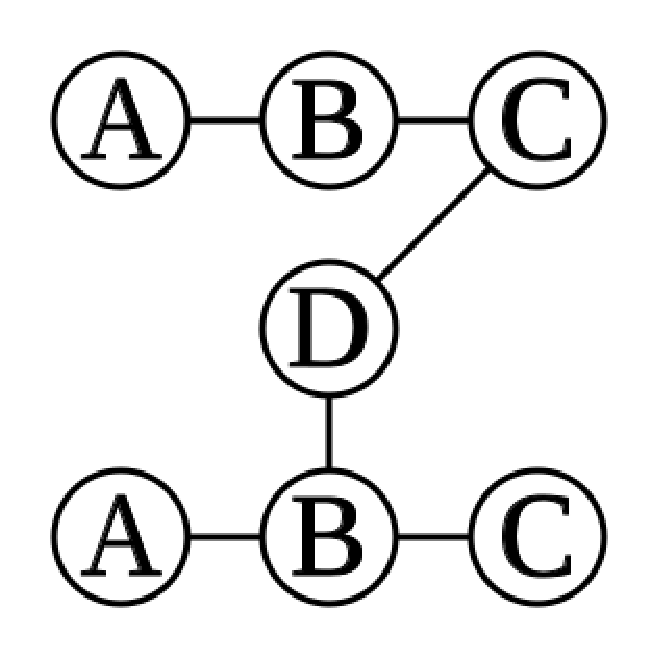
\includegraphics[width=0.4\textwidth]{img/artificial_graph/abc3abc2.eps} \\
						$y = -1$
					\end{minipage}
					\begin{minipage}{0.4\hsize}
						\centering
						\begin{tabular}{ll}
							\thickhline
							Group 1 & Group 2 \\
							\hline
							\gxxx{A}{A}{A} & \gxxx{B}{B}{B} \\
							\gxxx{C}{C}{C} & \gxxx{A}{A}{B} \\
							\gxxx{B}{C}{C} & \gxxx{A}{B}{C} \\
							\thickhline
						\end{tabular}
					\end{minipage} 
				\end{tabular}
			}
		\end{figure}

		\vspace{25pt}
		\begin{center}
			\express{非線形モデルが必要}
		\end{center}
		\begin{table}[t]
			\centering
			\scalebox{0.9}{
				\begin{tabular}{lll}
					\thickhline
					\multicolumn{1}{l}{\textit{非線形モデル}}~~~~~~~ &
					\multicolumn{2}{l}{\textit{線形モデル}} \\ \hline
					%Proposed & RF & Proposed ($d1$) & gBoost & LR \\
					提案手法 & 提案手法 ($d1$)~~~ & gBoost \\
					\hline
					%\fst{100.0} &  \scd{94.3}  & 64.3  & 70.0  & 53.9  \\
					~~\fst{100.0} & ~~~~64.3  & ~~70.0 \\
					\thickhline
				\end{tabular}
			}
		\end{table}
	\hspace{700pt} $d$: 木の深さ 

	\vspace{10pt}
	\structure{精度予測 (\%) QSAR} \\
	\vspace{-35pt}
	\begin{center}
		\express{実データに対しても高精度}
	\end{center}
	\begin{table}[t]
		\centering
		\scalebox{0.9}{
			\begin{tabular}{lcccc}
				\thickhline
				~                          &        CPDB                ~~~ &        Mutag             ~~~ &        NCI1               ~~~ &        NCI47                    \\ \hline
				\multicolumn{5}{l}{\textit{非線形モデル}} \\
				\ss{提案手法}{~}           &   \fss{79.3}   ~~~ &    \ss{87.8} ~~~ &   \fss{84.7}  ~~~ &   \fss{84.5}  ~~~   \\ \hline
				\multicolumn{5}{l}{\textit{線形モデル}} \\
				\ss{提案手法 (d1)}{~}      &    \fss{79.3}  ~~~ &    \ss{87.8} ~~~ &    \ss{83.1}  ~~~ &    \ss{82.8}  ~~~   \\
				\ss{gBoost}{~}             &    \ss{77.1}   ~~~ &   \fss{91.4} ~~~ &    \ss{82.7}  ~~~ &    \ss{81.3}  ~~~   \\
				\thickhline
			\end{tabular}
		}
	\end{table}

	\vspace{10pt}
	\structure{2-step 手法とのスケーラビリティの比較} \\
	\vspace{-35pt}
	\begin{center}
		\express{2-step手法よりもスケールする}
	\end{center}
	\begin{figure}[t]
		\centering
		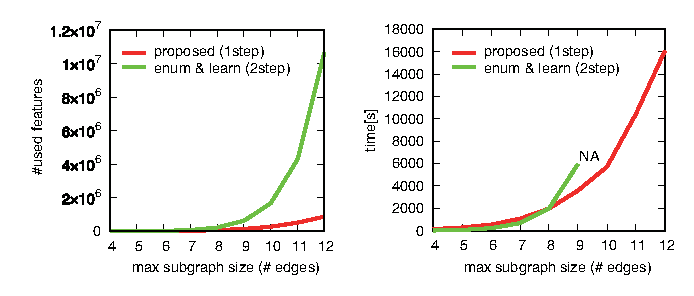
\includegraphics[width=1\textwidth]{img/fig7_panel.eps}
	\end{figure}
\end{tcolorbox}

	\end{column}
\end{columns}


\vspace{10pt}
\begin{beamercolorbox}[
		wd=1.01\textwidth,
		sep=0pt,     % パディング 2pt
	]{myframetitle}
	\begin{center}
		{\Large 提案手法} \\
	\end{center}
\end{beamercolorbox}
\vspace{12pt}

\fontsize{30pt}{0pt} \selectfont
\begin{columns}[T]
		\begin{column}{0.50\textwidth}
			\begin{tcolorbox}[colbacktitle=gray, title={\fontsize{35pt}{0pt}\selectfont 非線形グラフ分類回帰モデル}]
	\structure{回帰木} \\
	\vspace*{-10pt} 
	\vspace{-30pt} \\
\hspace*{720pt}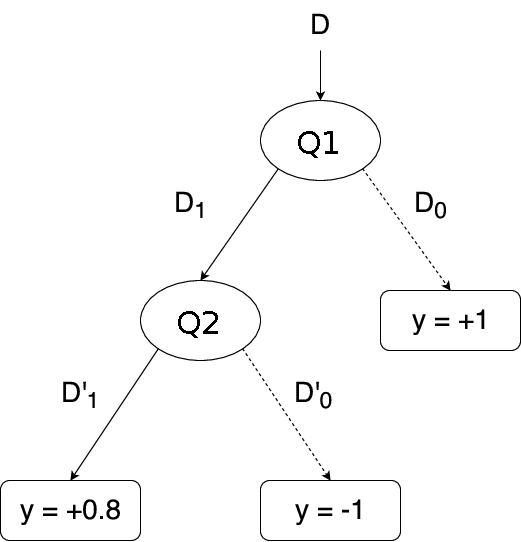
\includegraphics[width=300pt]{img/dtr_drawio.png}
\begin{textblock*}{\textwidth}(000pt,-440pt)
	\vspace*{160pt}
	入力データに対して \\
	内部ノードで質問し最適な分割を行う \\
	葉ノードで定数値を返す \\

	\vspace*{30pt}
	質問 : \\
	ある部分グラフを含むor含まない \\

	\vspace*{20pt}
\end{textblock*}
\begin{textblock*}{\textwidth}(875pt,-205pt)
	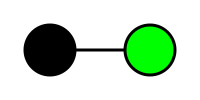
\includegraphics[width=60pt]{img/subgraph/kg.png}
\end{textblock*}
\begin{textblock*}{\textwidth}(750pt,-205pt)
	\scriptsize
	\fontsize{18pt}{0pt} \selectfont含む
\end{textblock*}
\begin{textblock*}{\textwidth}(990pt,-205pt)
	\scriptsize
	\fontsize{18pt}{0pt} \selectfont含まない
	\end{textblock*}
\begin{textblock*}{\textwidth}(815pt,-100pt)
	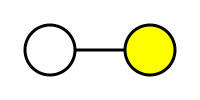
\includegraphics[width=60pt]{img/subgraph/wy.png}
\end{textblock*}
\begin{textblock*}{\textwidth}(700pt,-95pt)
	\scriptsize
	\fontsize{18pt}{0pt} \selectfont含む
\end{textblock*}
\begin{textblock*}{\textwidth}(930pt,-95pt)
	\scriptsize
	\fontsize{18pt}{0pt} \selectfont含まない
\end{textblock*}


	\vspace*{-20pt} 
	\structure{勾配ブースティング} \\
	\vspace*{5pt} \\
	加法的アンサンブルモデル
	\begin{equation}
		F(G) = T_0(G) + s T_1(G) + s T_2(G) + s T_3(G) + \cdots
	\end{equation}
	%\vspace{-30pt} \\
	$T_k$ : 各反復における残差$r_i$に対する回帰木.
	\begin{equation}
		r_i = \frac{\partial \mathrm{L}(y_i, F_{k-1}(G_i))}{\partial F}
	\end{equation}
	\color{ash}
	$s$ : 学習率, \hspace{10pt} $\mathrm{L}$ : 損失関数.
	\vspace*{20pt} 

	\color{black}
	\structure{内部ノードにおける分割ルールの学習} \\
	\vspace*{5pt} \\
	二乗誤差和を最小化する分割ルール(部分グラフ)の学習
	\begin{equation}
		\arg\mymin{x_j \in X} \big[ \TSS(D_1(x_j)) + \TSS(D_0(x_j)) \big]
		\label{min:internal}
		\vspace{-5pt}
	\end{equation}
	$X$ : 全部分グラフ集合(\alert{全列挙は困難}) \\
	$D_1(x_j)$ : $ \{x_j$を含むグラフ集合$\}$, \hspace{30pt} $D_0(x_j)$ : $ \{x_j$を含まないグラフ集合$\}$ \\
	$\TSS(D)$ : 残差$r_i$に対する二乗誤差和 \\
	\vspace{-10pt}
\end{tcolorbox}

		\end{column}
		\begin{column}{0.50\textwidth}
			\begin{tcolorbox}[colbacktitle=gray, title={\fontsize{35pt}{0pt}\selectfont 内部ノードにおける分割ルールの学習}]
	\structure{探索空間} \\
\end{tcolorbox}

		\end{column}
\end{columns}
\fontsize{22pt}{0pt} \selectfont{
Jointly Learning Relevant Subgraph Patterns and Nonlinear Models of Their Indicators.
The 14th International Conference on Mining and Learning with Graphs (MLG 2018), KDD'18 Workshop, London, U.K., August 20, 2018
}

\end{document}
